\chapter{Metodi reattivi per il controllo}
\label{chap:chap2}

Questo capitolo si occupa di descrivere la navigazione con 
\textit{metodi reattivi}, in quanto rappresenta una strategia largamente 
utilizzata per il controllo di un agente autonomo. 
Essa suggerisce di prendere tutte le decisioni di controllo attraverso
un'elaborazione dei dati recenti dei sensori. 
Infatti, sono algoritmi senza un vero e proprio piano che cercano di guidare il veicolo 
evitando gli ostacoli o seguendo un percorso prestabilito -- spesso generato 
dal modulo di \textit{planning}, come spiegato nella sottosezione~\ref{subs:planning} --
fornendo input di sterzata e velocità all’auto per effettuare manovre fluide.

\section{PID Controller}
% Reactive di tipo longitudinale: determina la velocità
Una strategia semplice per far navigare l'auto consiste nel seguire una linea 
(\textit{line follow}), un muro di un corridoio o il cordolo di un circuito (\textit{wall follow}), 
attraverso un \textit{controllore} che fornisce input di \textit{sterzata} e 
\textit{accelerazione} all'auto autonoma. 

L'algoritmo più diffuso che fornisce questi input è il controllore \textit{PID},
acronimo di \textit{Proportional, Integral e Derivative}.
Si tratta di un controller molto popolare e versatile, il cui punto di forza risiede nella
sua semplicità e nei risultati che ottiene. Questo tipo di controller viene usato
nelle applicazioni che richiedono un controllo di tipo \textit{closed-loop feedback}.
Di seguito si descrive come il controllore calcola l'angolo di sterzata e la velocità
a cui guidare per poter eseguire una manovra \textit{fluida}.
\subsection{Struttura}
Il controllore acquisisce in ingresso un valore e lo confronta con un valore di 
riferimento, detto \textit{setpoint}. La differenza tra questi due valori corrisponde 
al segnale di \textit{errore}, che viene usato per determinare il valore di uscita del controllore.

Il controller \textit{PID} regola l’uscita in base ai seguenti parametri:
\begin{enumerate}
    \item il valore del segnale di errore (azione proporzionale);
    \item la somma degli errori accumulati nel tempo fino all'istante corrente (azione integrale);
    \item la velocità di variazione del segnale di errore (azione derivata).
\end{enumerate}

\begin{figure}[H]
    \centering
    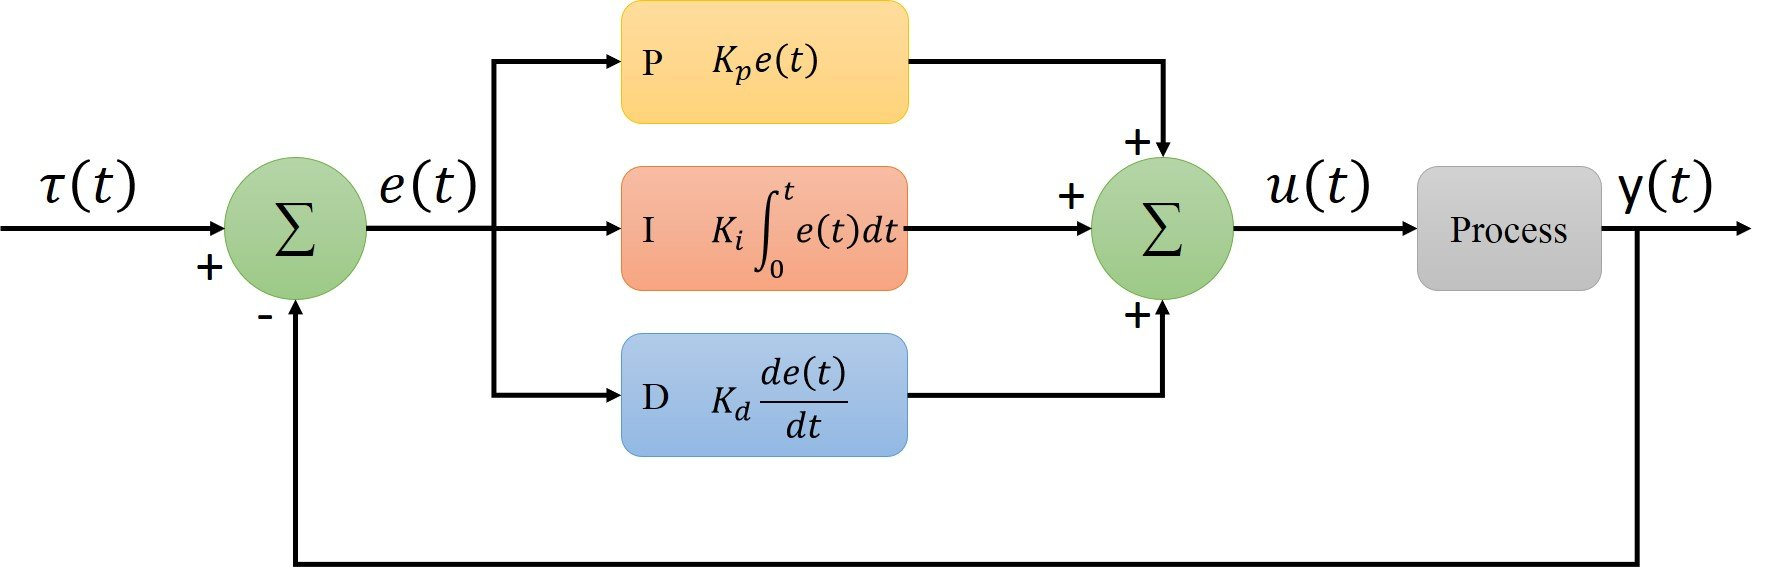
\includegraphics[width=\textwidth]{images/PID_controller.jpg}
    \caption{Schema a blocchi del PID controller. Qui $\tau(t)$ è il setpoint, $u(t)$ è l'output di controllo, mentre $y(t)$ è il valore della variabile di processo~\cite{pidimg}.}
    \label{fig:fig7} % etichetta utilizzata per riferisi all'immagine
\end{figure}
Nello specifico, le componenti di controllo del \textit{PID} sono:
\begin{itemize}
    \item \verb|Proportional Controller| -- l'angolo di sterzata dell'auto deve essere proporzionale 
    alla distanza della stessa dal percorso stabilito, detta \textit{crosstrack error}. 
    Maggiore è l’errore, maggiore deve essere la correzione per correggerlo.
    \item \verb|Derivative Controller| -- lo svantaggio principale del \verb|Proportional|
    è che provoca continue oscillazioni attorno alla linea centrale e aumenta 
    l'\textit{overshoot}, cioè il superamento del \textit{setpoint}. 
    Quello che si desidera, invece, è che l'errore diminuisca nel tempo, riducendo di 
    conseguenza anche l'azione correttiva.
    Prevenendo quest'effetto, si applica una correzione anticipata, che deve essere
    proporzionale alla velocità con cui l’errore si sta riducendo.
    Una previsione triviale è data dall’attuazione di un \verb|gain| basato sull’errore, che
    porterà il robot a controsterzare e ad avvicinarsi progressivamente alla linea centrale. 
    Dunque, l'azione derivata prevede il comportamento del sistema e ne migliora la stabilità.
    \item \verb|Integral Controller| -- è possibile includere anche un termine di 
    \verb|gain| integrale, che è proporzionale all’errore accumulato a partire da un tempo
    di riferimento $t$. L'azione integrale, dunque, tiene conto del \textit{crosstrack error} 
    accumulato nel tempo, correggendo gli errori che non sono stati risolti nei passi temporali precedenti.
\end{itemize}
L'output di controllo $u(t)$ di quest'algoritmo, vale a dire ciò che viene controllato, è 
l'angolo di sterzata $\delta$ a cui si vuole che l'auto guidi. 
Si può così indicare di seguito l'equazione standard di \textit{PID}, dove $e(t)$ è 
l'errore dalla traiettoria desiderata:
\[
u(t) = K_p e(t) + K_d \frac{de(t)}{dt} + K_i \int_{0}^{t} e(t) \,dt
\]
Le \textit{costanti} $K_p$, $K_i$ e $K_d$ determinano con quale peso contribuisce ciascuna delle tre componenti.
Nell'implementazione di PID, l'azione \textit{integrale} non è sempre necessaria.
Infatti, a seguito di una grande variazione del \textit{setpoint}, il termine integrale
può accumulare un errore superiore al valore massimo della variabile di controllo,
portando il sistema in \textit{overshooting}, con conseguente aumento dell'errore.
La soluzione a questo problema consiste nel disabilitare l'azione integrale~\cite{f1tenthcoursel04}.

Ricapitolando, il \verb|Proportional| svolge la maggior parte del lavoro, 
il \verb|Derivative| agisce sul primo per ridurne l'\textit{overshoot} e 
l'\verb|Integral|, se presente, riduce l'errore che resta dopo che il primo ha svolto il suo lavoro.

\subsection{Tuning}
Il \textit{PID} è un esempio di metodo di controllo libero da qualsiasi tipo di \textit{modello}: 
non si modella il veicolo e quindi, per ottimizzare i valori dei \verb|gain| di controllo 
$K_p$, $K_i$ e $K_d$, bisogna fare affidamento sull'esperienza e sull'analisi.
Un ingegnere del controllo deve sapere cosa si può fare, cosa non è sicuro e quali bias
sono presenti nel sistema, tuttavia molto dipende anche dalle caratteristiche prestazionali desiderate. 
Esistono sia approcci manuali che euristiche, come quella di \textit{Ziegler-Nichols}. Nell'ambito di F1TENTH, il metodo più comune è quello manuale, soprattutto in ambiente 
simulativo, come in questo caso. Con un divario inferiore tra la simulazione e la realtà 
(\textit{Sim2Real}), il codice sviluppato nel simulatore potrebbe essere utilizzato direttamente sull'auto reale.

\section{Pure Pursuit}
Il metodo del \textit{Pure Pursuit} è uno degli approcci più diffusi nella guida
autonoma per il problema affrontato in questa tesi: il \textit{path tracking} per
auto autonome da corsa.
Al veicolo viene assegnata una sequenza di posizioni da seguire, dette \textit{waypoint},
indicate nel frame di riferimento del veicolo e l'obiettivo dell'algoritmo consiste nel seguirli.

Il controllo del movimento di un veicolo \textit{olonomico} è più semplice: essi possono muoversi in 
qualsiasi direzione, a prescindere dall'orientamento del veicolo. Tuttavia, in questo contesto si ha un
veicolo non olonomico, cioè l'automobile di \textit{F1TENTH}, che deve riposizionarsi e cambiare direzione per spostarsi in un 
certo punto. Ciò, infatti, complica il problema del \textit{path tracking}.

Per affrontare questa sfida, \textit{Pure Pursuit} calcola geometricamente 
la curvatura di un arco che collega la posizione dell'asse posteriore dell'auto a un punto di 
\textit{goal} sul percorso da seguire. Quest'ultimo è sempre il \textit{waypoint} più vicino
al veicolo e ad almeno una data distanza di \textit{lookahead}, che va dalla posizione corrente
dell'auto al percorso desiderato.
In questo contesto, \textit{Pure Pursuit} rappresenta un controller laterale che ignora le 
forze dinamiche che agiscono sui veicoli e presuppone che le ruote mantengano la condizione 
antiscivolo (\textit{no-slip}).

L'algoritmo è un \verb|P Controller| dell'angolo di sterzata $\delta$ che agisce sull'errore
di tracking, secondo un certo \verb|gain| e \textit{lookahead}. 
%In breve, il puro controllo dell'inseguimento funziona come un controllore proporzionale dell'angolo di sterzata agendo sull'errore di traslazione
Per determinare l'angolo, si calcola come segue la curvatura dell'arco $\gamma$:
\begin{equation}
    r = \frac{L^2}{2|y|} \rightarrow \gamma = \frac{1}{r} = \frac{2|y|}{L^2}
\end{equation}
Il \textit{lookahead} è sempre soggetto a operazioni di \textit{tuning}: 
con un valore basso si ha un tracciamento più accurato, ma più oscillazioni;
invece se più alto, si osservano meno oscillazioni, ottenendo però un peggioramento del 
tracciamento. Infine, viene attuata la velocità che è indicata per ogni waypoint del percorso.
%\textit{Pure Pursuit} è un controller per il path tracking geometrico che si basa sul nostro modello di veicolo per selezionare i comandi di sterzata.
%Quest'algoritmo è stato originariamente concepito come metodo di controllo per calcolare l'arco necessario per riportare un robot su un percorso.
\section{Vantaggi e svantaggi}
I \textit{vantaggi} dei \textit{metodi reattivi per il controllo} comprendono: 
\begin{enumerate}
    \item la possibilità di applicarlo a robot con risorse hardware limitate e a basso prezzo;
    \item il fatto di poter far navigare un robot in sicurezza in ambienti completamente 
    sconosciuti e contenenti ostacoli non prevedibili.
\end{enumerate}
Invece, tra gli \textit{svantaggi} di questi metodi si ha che:
\begin{enumerate}
    \item possono occasionalmente far seguire traiettorie \textit{impraticabili} per i robot, 
    dunque non è facile adattarli a sistemi più complessi;
    \item i \verb|gain| di controllo devono essere regolati manualmente e per diverso tempo, 
    comportando un'intensa attività di \verb|tuning|;
    \item un'eventuale suddivisione del problema in due diversi controllori 
    (\textit{longitudinale} e \textit{laterale}) ignorerebbe l'accoppiamento tra le due 
    dimensioni. Ciò comporterebbe che, per esempio, il controllore \textit{PID}, usato solo 
    come controllore longitudinale, non sappia nulla del controllore laterale 
    (\textit{Pure Pursuit}). In certe situazioni, come in una curva, ciò può generare problemi nella sterzata;
    \item non offrono alcuna possibilità di gestione dei vincoli;
    \item considerano solo lo stato attuale e, dunque, ignorano le decisioni future. In questo modo, non considerano le conseguenze che possono avere le decisioni attuali sulle successive.
\end{enumerate}
Come anticipato nella sottosezione~\ref{subs:control}, \textit{Model Predictive Control} 
costituisce una soluzione più avanzata che permette di superare i limiti dei metodi reattivi, 
poiché ha alla base il \textit{controllo ottimale}.